
正如记录需求一样,也应该记录出现的架构。这当然不仅仅是为了拥有文档,它应该帮助每个参与项目的人提高生产力,使他们更好地理解自己的角色和最终产品需要什么。并不是所有的图表都对每个人都有用,但是可以试着从未来读者的角度来创建它们。

有许多框架可以记录愿景,其中许多框架服务于特定的领域、项目类型或体系结构范围。例如,如果对记录企业架构感兴趣,那么可能会对TOGAF感兴趣。这是\textit{开放组架构框架}的首字母缩写。它依赖于四个领域,即:

\begin{itemize}
\item 
业务架构(策略、组织、关键流程和治理)

\item 
数据架构(逻辑和物理数据管理)

\item 
应用架构(单系统的蓝图)

\item
技术架构(硬件、软件和网络基础设施)
\end{itemize}

如果将软件记录放在整个公司,甚至更广泛的范围内,那么这种分组就很重要。其他类似规模的框架包括由\textbf{英国国防部(MODAF)}和\textbf{美国等效机构(DoDAF)}开发的框架。

如果没有记录企业架构,若是刚刚开始架构自我开发道路,可能会对其他框架更感兴趣,例如4+1和C4模型。

\subsubsubsection{3.6.1\hspace{0.2cm}4+1模型}

4+1模型是由Philippe Kruchten在1995年创建。然后,作者称它旨在“对多个并发视图的使用,描述软件密集型系统的架构”。它的名字来自于它所包含的视图。

这种模型已经在市场上存在了很长时间,也非常有效果,因此广为人知。它非常适合于大项目,当然也可以用于中小型的项目,但对于需求来说也可能过于复杂(特别是用敏捷的方式编写的)。如果正处于这种情况,应该尝试下一节中的C4模型。

4+1模型的缺点是它使用了一组固定的视图,而文档体系结构需要根据项目的具体情况选择视图(稍后将详细介绍)。

优点是可以清晰的了解视图是如何连接在一起,特别是涉及到场景时。同时,每个责任方可以很容易地了解与他们相关的部分。来展示一下模型:

\begin{center}
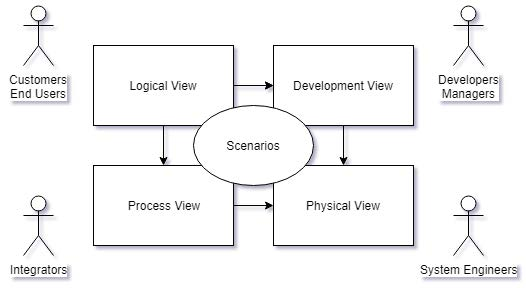
\includegraphics[width=0.6\textwidth]{content/1/chapter3/images/1.jpg}\\
图3.1 - 4+1模式概览
\end{center}

上图中的参与者对其对应的视图最感兴趣。所有的视图都可以用不同种类的\textbf{统一建模语言(UML)}图来表示。现在了解下每个视图:

\begin{itemize}
\item 
\textbf{逻辑视图}展示了如何向用户提供功能,以及系统的组件(对象)如何交互。最常见的是,它由类和状态图组成。如果有成千上万的类或者只是想更好地显示交互,应该有通信图或序列图,两者都是下个视图的一部分:

\begin{center}
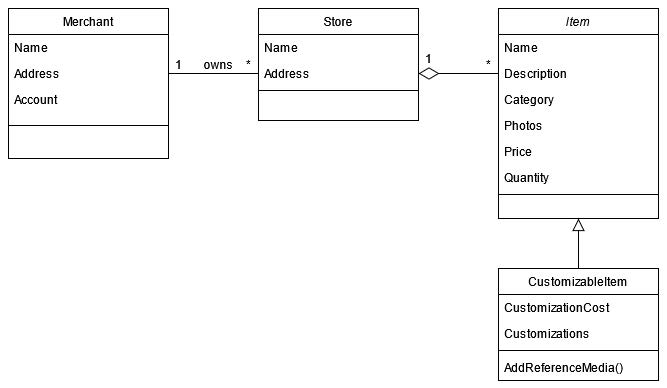
\includegraphics[width=0.7\textwidth]{content/1/chapter3/images/2.jpg}\\
图3.2 -类图可以用来显示计划拥有的类型,以及它们的关系
\end{center}

\item 
\textbf{进程视图}围绕着系统的运行时行为,显示进程、进程之间的通信以及与外部系统的交互,由活动和交互图表示。此视图处理许多NFR,包括并发性、性能、可用性和可扩展性:

\begin{center}
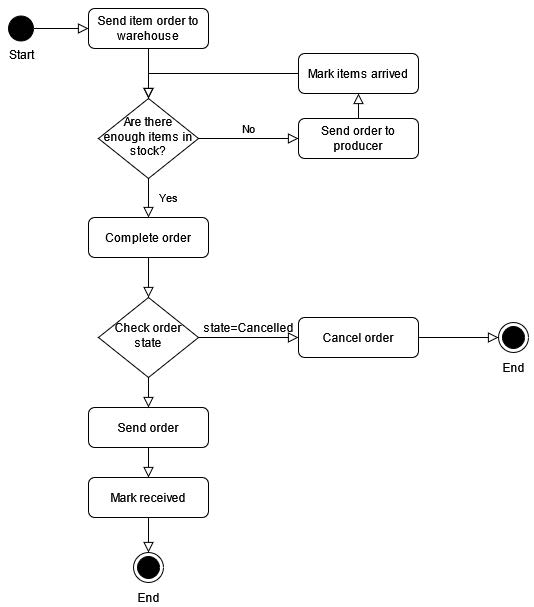
\includegraphics[width=0.6\textwidth]{content/1/chapter3/images/3.jpg}\\
图3.3 -活动图工作流和过程的图形表示
\end{center}

\item 
\textbf{开发视图}为了分解成子系统,并围绕着软件组织。重用、工具约束、分层、模块化、打包、执行环境——这个视图可以通过显示系统的构建块来表示它们。通过使用组件和包图来实现:

\begin{center}
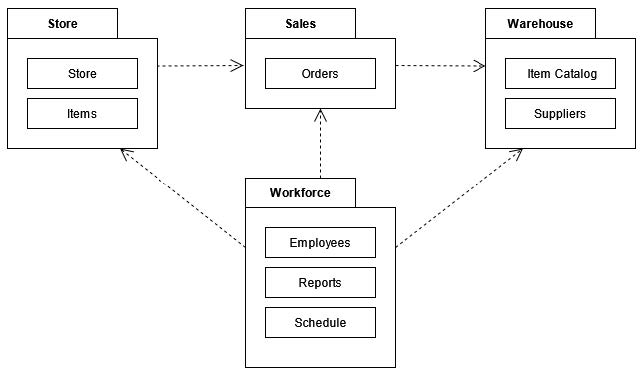
\includegraphics[width=0.8\textwidth]{content/1/chapter3/images/4.jpg}\\
图3.4 -包图可以从更高的角度显示系统的各个部分,以及特定组件之间的依赖关系
\end{center}

\item
\textbf{物理视图}使用部署图将软件映射到硬件。针对系统工程师,可以涵盖与硬件相关的NFR子集,例如通信:

\begin{center}
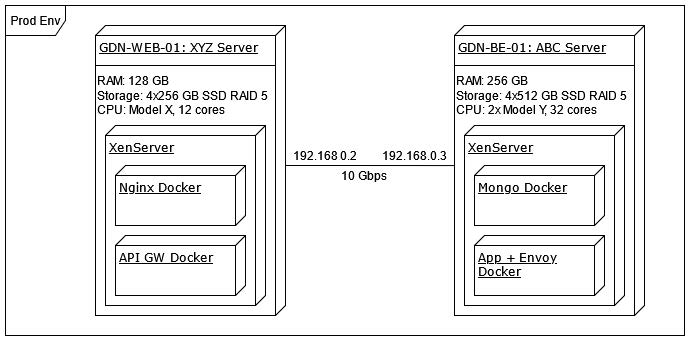
\includegraphics[width=0.9\textwidth]{content/1/chapter3/images/5.jpg}\\
图3.5 -部署图展示了运行每个软件组件的硬件,还可以用来传递有关网络的信息
\end{center}

\item
\textbf{场景视图}把所有其他的视图都连接在一起,这些对所有相关方都是有用的。这个视图可以显示系统是否做了它应该做的事情。当其他视图都完成后,场景视图可能是多余的。但是,如果没有使用场景,所有其他视图都是不可能完成。这个视图从高层次展示了系统,而其他视图则展示了更多的细节:

\begin{center}
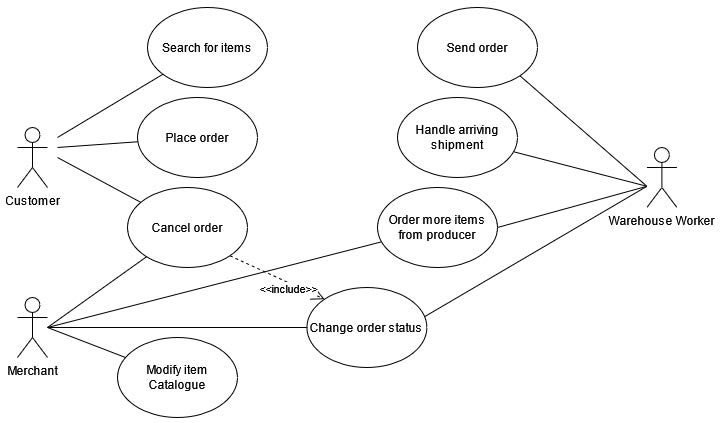
\includegraphics[width=0.9\textwidth]{content/1/chapter3/images/6.jpg}\\
图3.6 -用例图显示了特定的参与者如何与系统交互,以及如何交互,彼此关联
\end{center}

\end{itemize}

这些视图中的每一个都与其他视图相互关联,通常必须共存才能显示出全貌。需要考虑下,如何表达并发。它不能只使用逻辑视图来完成,因为将其映射到任务和流程更有表现力,从而需要过程视图。另一方面,进程将映射到物理(通常是分布式的)节点。这意味着需要在三个视图中进行记录,每个视图都与特定的责任方相关。视图之间的其他连接包括:

\begin{itemize}
\item
逻辑视图和过程视图都用于分析和设计,以概念化产品。

\item 
将开发和部署结合在一起,描述了软件是如何打包的,以及每个包将在何时部署。

\item
逻辑视图和开发视图显示了功能是如何反映在源码中。

\item
流程和部署视图共同描述NFR。
\end{itemize}

熟悉了4+1模型,继续了解另一个简单但非常有效的模型:C4模型。希望使用它将是一个爆炸(双关语[译注:关联的是著名的C4炸弹])。

\subsubsubsection{3.6.2\hspace{0.2cm}C4模型}

C4模型非常适合中小型项目。因为简单,所以很容易应用,并且不依赖于任何预定义的符号。如果想用它来绘制图表,可以试试Tobias Shochguertel的c4-draw.io插件(\url{https://github.com/tobiashochguertel/c4-draw.io})的免费在线绘图工具-draw.io(\url{https://www.draw.io/})。

在C4模型中,主要有四种图类型,即:

\begin{itemize}
\item
系统上下文

\item 
容器

\item
组件

\item
代码
\end{itemize}

就像使用地图放大和缩小一样,可以使用这四种类型来显示特定代码区域的细节,或者“缩小”来显示关于特定模块,甚至整个系统的交互和周围环境的更多信息。

系统上下文是查看架构的一个很好的起点,因为它将系统作为一个整体显示出来,周围是与其交互的用户和其他系统。可以在这里看到一个C4模型的上下文关系图:

\begin{center}
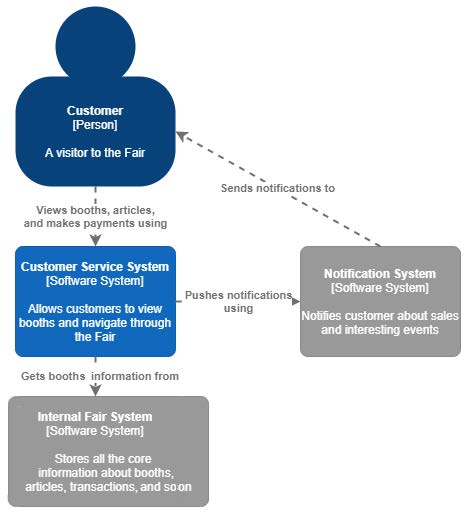
\includegraphics[width=0.9\textwidth]{content/1/chapter3/images/7.jpg}\\
图3.7 - C4上下文关系图
\end{center}

它展示了“大局”,所以它不应该专注于特定的技术或协议。相反,可以把它看作是可以向非技术相关方展示的图表。仅通过查看图表,就可以清楚地看到有一个参与者(对客户的人形描述),他与解决方案的一个组件(即客户服务系统)交互。另一方面,这个系统与另外两个系统相互作用,每个相互作用都用箭头表示。

上下文关系图用于提供系统的概览,其中包含一些细节。现在让逐一查看其他图表:

\begin{itemize}
\item
\textbf{容器图}: 用来显示系统内部的概述。如果系统使用数据库,提供服务,或者只是由某些应用程序组成,则此图将显示它。还可以展示容器的主要技术选择。注意,容器不是指Docker容器,尽管每个图都是单独的可运行和部署单元,但此图类型与部署场景无关。容器视图是为技术人员设计的,但并不仅限于开发团队。架构师以及操作和支持人员也是目标受众。

\item 
\textbf{组件图}: 如果想要关于特定容器的更多细节信息,就需要组件图发挥作用了。它展示了所选容器内的组件如何彼此交互,以及如何与容器外的元素和参与者交互。通过查看这张图,可以了解每个组件的职责,以及使用什么技术构建它。组件图的目标受众主要集中在一个特定的容器上,由开发团队和架构师组成。

\item
\textbf{代码图}: 最后来看代码图,将组件放大到一定程度时,代码图就会出现。这个视图主要由UML图组成,包括类、实体关系和其他,理想情况下应该由独立的工具和IDE从源代码自动创建。绝对不应该为系统中的每个组件制作这样的关系图;相反,把重点放在最重要的内容上,让它们告诉读者架构想要表达的内容。想要这样的图中少一些,就要从代码图中删掉不必要的元素。在许多系统中,特别是在较小的系统中,这类图会直接省略。目标受众与组件图中的受众相同。
\end{itemize}

可能会发现C4模型缺少一些特定的视图。例如,如果想知道如何演示应该如何部署系统,可能会有兴趣了解除了主图之外,还有一些补充图。其中之一是部署图,它展示了如何将系统中的容器映射到基础设施中的节点。通常,其是UML部署图的一个简单版本:

\begin{center}
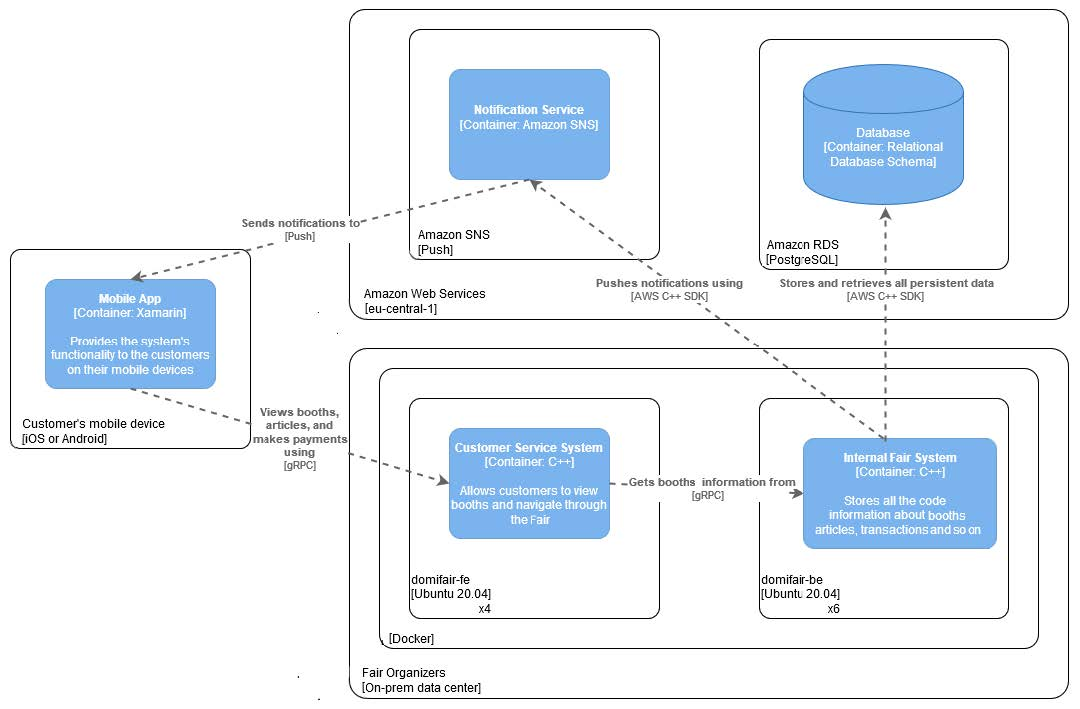
\includegraphics[width=0.9\textwidth]{content/1/chapter3/images/8.jpg}\\
图3.8 - C4部署图
\end{center}

说到与C4模型相关的UML图,可能还要知道为什么它在展示系统的用例上投入了这么少的努力。如果遇到了这种情况,那么应该考虑使用UML的用例图来补充前面的模型,或者可能考虑引入一些序列图。

在记录架构时,记录的内容和共享的知识比遵循特定的硬性规则更重要。可以选择最适合的工具。

\subsubsubsection{3.6.3\hspace{0.2cm}记录敏捷项目中的架构}

敏捷环境中,记录架构的方法应该与记录需求的方法类似。首先,考虑谁会阅读这些材料,确保以正确的方式描述了正确的事情。文档不需要是一个冗长的Word文档。当有人描述架构时,可以使用演示文稿、Wiki页面、单个图表,甚至是会议的录音进行记录。

重要的是收集关于文档化架构的反馈。与文档化的需求一样,重要的告知相关方文档更新,以便器了解都改进了哪里。尽管这看起来像是在浪费时间,但如果处理得当,会为你节省交付产品的时间。足够好的文档可以帮助新手快速开始工作,并指导更熟悉的责任人。如果只是在一些会议上讨论架构,那么很有可能,会议之后就没有人会记得出于什么原因才做出的那些决策,以及这些决策在不断变化的敏捷环境中是否仍然有效。

创建文档时,重复阅读是很重要的,因为很可能会对一两个重要的细节有一些误解。其他时候,架构师或相关方会了解更多的东西,从而对原有的决定进行更改。在文件认为是成熟和完成之前,至少要准备好把它们多看几遍。通常,通过即时通讯工具、电话或面对面的交谈可以更快地完成任务,并解决可能出现的后续问题,所以比起电子邮件或其他异步的沟通方式,架构师可能会更喜欢这些方式。


























